%%%%%%%%%%%%%%%%%%%%%%%%%%%%%%%%%%%%%%%%%
% Beamer Presentation
% LaTeX Template
% Version 1.0 (10/11/12)
%
% This template has been downloaded from:
% http://www.LaTeXTemplates.com
%
% License:
% CC BY-NC-SA 3.0 (http://creativecommons.org/licenses/by-nc-sa/3.0/)
%
%%%%%%%%%%%%%%%%%%%%%%%%%%%%%%%%%%%%%%%%%

%----------------------------------------------------------------------------------------
%   PACKAGES AND THEMES
%----------------------------------------------------------------------------------------

\documentclass{beamer}

\mode<presentation> {
	
	% The Beamer class comes with a number of default slide themes
	% which change the colors and layouts of slides. Below this is a list
	% of all the themes, uncomment each in turn to see what they look like.
	
	%\usetheme{default}
	%\usetheme{AnnArbor}
	%\usetheme{Antibes}
	%\usetheme{Bergen}
	%\usetheme{Berkeley}
	%\usetheme{Berlin}
	%\usetheme{Boadilla}
	%\usetheme{CambridgeUS}
	%\usetheme{Copenhagen}
	%\usetheme{Darmstadt}
	%\usetheme{Dresden}
	%\usetheme{Frankfurt}
	%\usetheme{Goettingen}
	%\usetheme{Hannover}
	%\usetheme{Ilmenau}
	%\usetheme{JuanLesPins}
	%\usetheme{Luebeck}
	\usetheme{Madrid}
	%\usetheme{Malmoe}
	%\usetheme{Marburg}
	%\usetheme{Montpellier}
	%\usetheme{PaloAlto}
	%\usetheme{Pittsburgh}
	%\usetheme{Rochester}
	%\usetheme{Singapore}
	%\usetheme{Szeged}
	%\usetheme{Warsaw}
	
	% As well as themes, the Beamer class has a number of color themes
	% for any slide theme. Uncomment each of these in turn to see how it
	% changes the colors of your current slide theme.
	
	%\usecolortheme{albatross}
	%\usecolortheme{beaver}
	%\usecolortheme{beetle}
	%\usecolortheme{crane}
	%\usecolortheme{dolphin}
	%\usecolortheme{dove}
	%\usecolortheme{fly}
	%\usecolortheme{lily}
	%\usecolortheme{orchid}
	%\usecolortheme{rose}
	%\usecolortheme{seagull}
	%\usecolortheme{seahorse}
	%\usecolortheme{whale}
	%\usecolortheme{wolverine}
	
	%\setbeamertemplate{footline} % To remove the footer line in all slides uncomment this line
	%\setbeamertemplate{footline}[page number] % To replace the footer line in all slides with a simple slide count uncomment this line
	
	%\setbeamertemplate{navigation symbols}{} % To remove the navigation symbols from the bottom of all slides uncomment this line
}

\usepackage{graphicx} % Allows including images
\usepackage{booktabs} % Allows the use of \toprule, \midrule and \bottomrule in tables
\usepackage{pdfpages}


%----------------------------------------------------------------------------------------
%   TITLE PAGE
%----------------------------------------------------------------------------------------

\title[Meeting 1]{Meeting 1: Enumeration and Heuristics} % The short title appears at the bottom of every slide, the full title is only on the title page

\author{Stefan Gugler} % Your name
\institute[MIT] % Your institution as it will appear on the bottom of every slide, may be shorthand to save space
{
	Massachusetts Institute of Technology \\ % Your institution for the title page
	\medskip
	\textit{sgugler@mit.edu} % Your email address
}
\date{\today} % Date, can be changed to a custom date

\begin{document}
	
	\begin{frame}
	\titlepage % Print the title page as the first slide
\end{frame}

%\begin{frame}
%\frametitle{Overview} % Table of contents slide, comment this block out to remove it
%\tableofcontents % Throughout your presentation, if you choose to use \section{} and \subsection{} commands, these will automatically be printed on this slide as an overview of your presentation
%\end{frame}

%----------------------------------------------------------------------------------------
%   PRESENTATION SLIDES
%----------------------------------------------------------------------------------------

%------------------------------------------------
%\section{First Section} % Sections can be created in order to organize your presentation into discrete blocks, all sections and subsections are automatically printed in the table of contents as an overview of the talk
%------------------------------------------------

%\subsection{Subsection Example} % A subsection can be created just before a set of slides with a common theme to further break down your presentation into chunks

\begin{frame}
\frametitle{Mono-Heavy-Atomic Isoelectronic Ligand Distribution}
\begin{figure}[ht] 
	\label{ fig7} 
	\begin{minipage}[b]{0.5\linewidth}
		\centering
		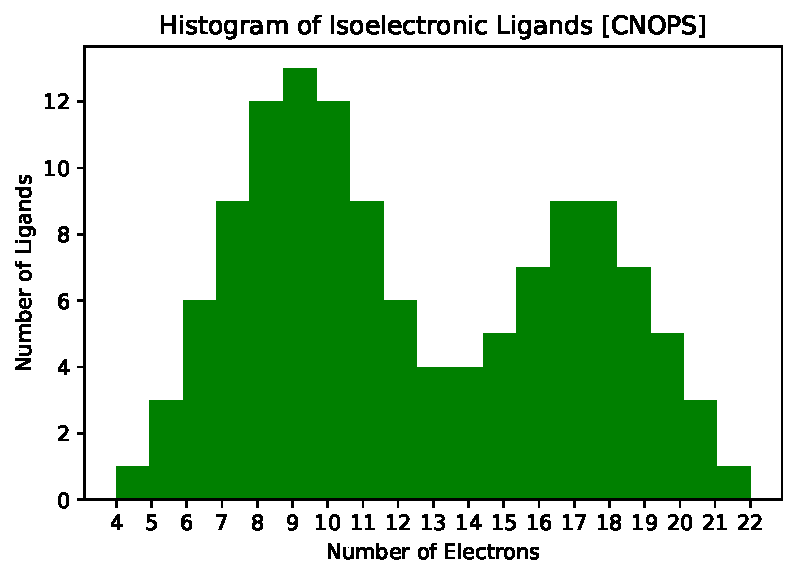
\includegraphics[width=.5\linewidth]{img/hist_iso_ligands_CNOPS.pdf} 
		\caption{CNOPS: 15625 ligands} 
		\vspace{4ex}
	\end{minipage}%%
	\begin{minipage}[b]{0.5\linewidth}
		\centering
		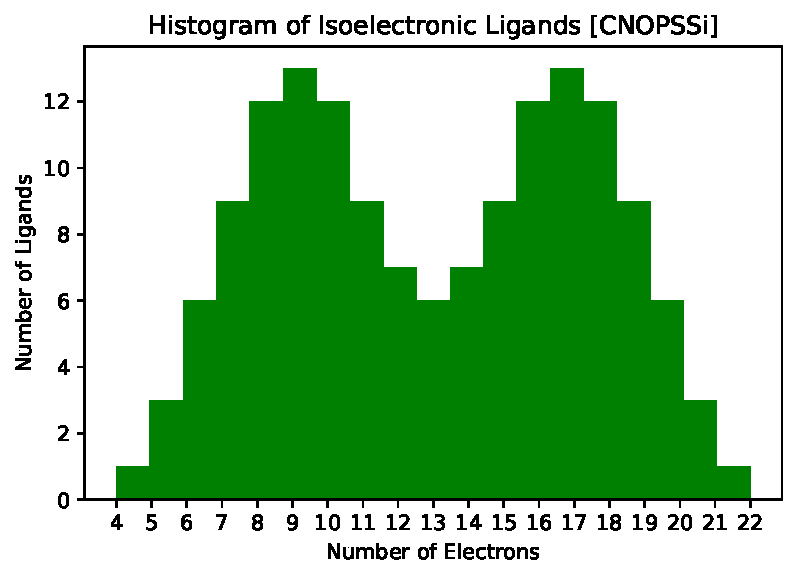
\includegraphics[width=.5\linewidth]{img/hist_iso_ligands_CNOPSSi.pdf} 
		\caption{CNOPSSi: 22500 (?) ligands} 
		\vspace{4ex}
	\end{minipage} 
	\begin{minipage}[b]{0.5\linewidth}
		\centering
		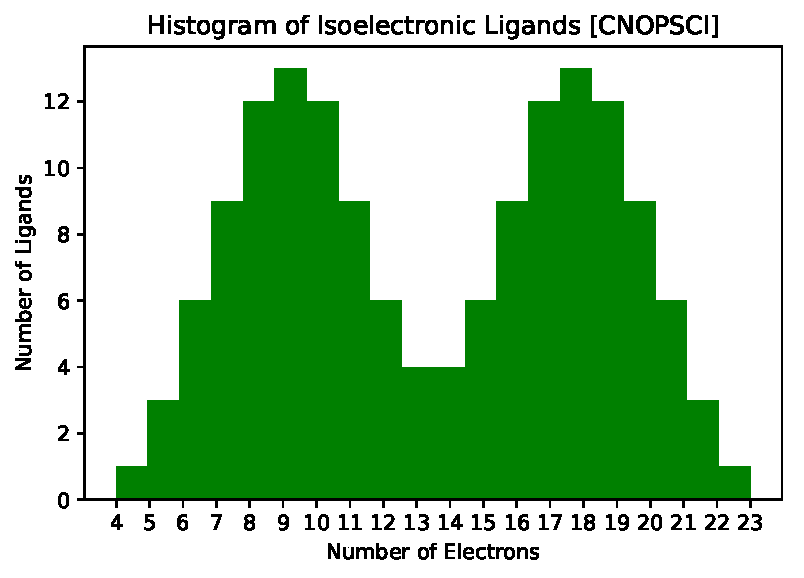
\includegraphics[width=.5\linewidth]{img/hist_iso_ligands_CNOPSCl.pdf} 
		\caption{CNOPSCl: 22500 (?) ligands} 
		\vspace{4ex}
	\end{minipage}%% 
	\begin{minipage}[b]{0.5\linewidth}
		\centering
		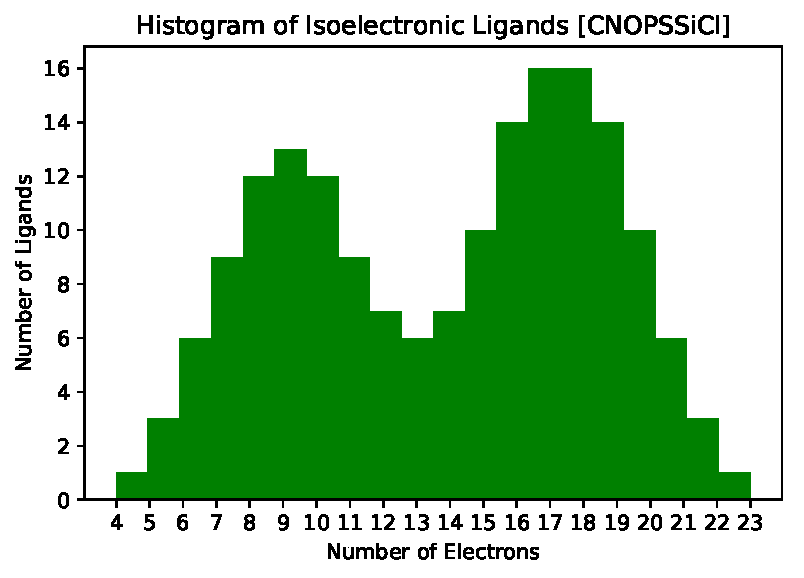
\includegraphics[width=.5\linewidth]{img/hist_iso_ligands_CNOPSSiCl.pdf} 
		\caption{CNOPSSiCl: 30625 ligands} 
		\vspace{4ex}
	\end{minipage} 
\end{figure}
\end{frame}

%------------------------------------------------

\begin{frame}
\frametitle{Mono-Heavy-Atomic Iso-VE Ligand Distribution}
\begin{figure}[ht] 
	\label{ fig7} 
	\begin{minipage}[b]{0.5\linewidth}
		\centering
		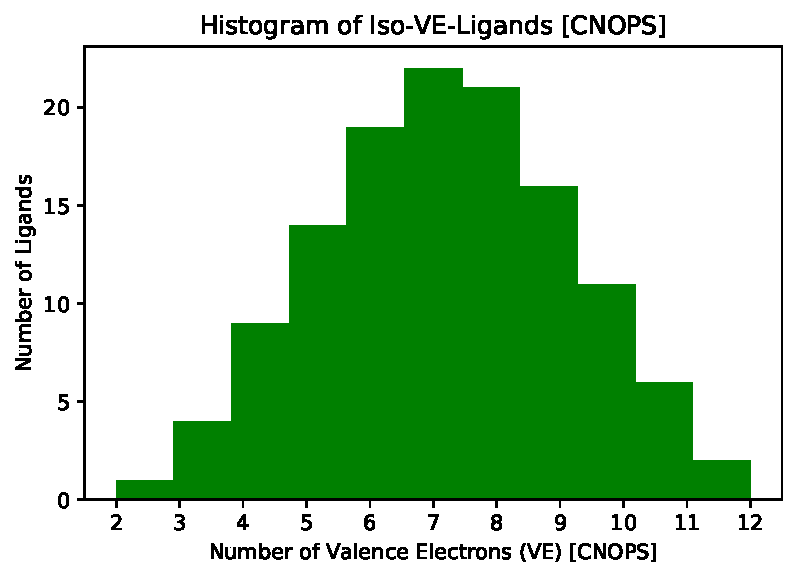
\includegraphics[width=.5\linewidth]{img/hist_isove_ligands_CNOPS.pdf} 
		\caption{CNOPS: 15625 ligands} 
		\vspace{4ex}
	\end{minipage}%%
	\begin{minipage}[b]{0.5\linewidth}
		\centering
		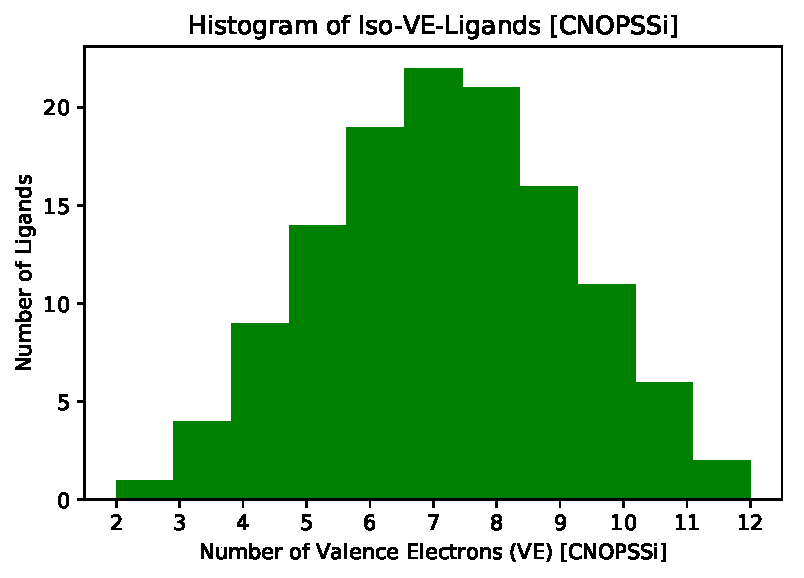
\includegraphics[width=.5\linewidth]{img/hist_isove_ligands_CNOPSSi.pdf} 
		\caption{CNOPSSi: 22500 (?) ligands} 
		\vspace{4ex}
	\end{minipage} 
	\begin{minipage}[b]{0.5\linewidth}
		\centering
		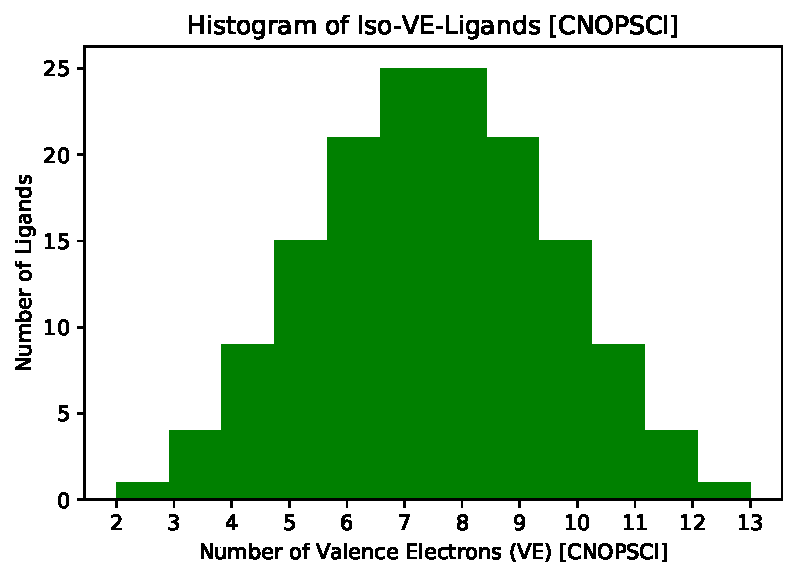
\includegraphics[width=.5\linewidth]{img/hist_isove_ligands_CNOPSCl.pdf} 
		\caption{CNOPSCl: 22500 (?) ligands} 
		\vspace{4ex}
	\end{minipage}%% 
	\begin{minipage}[b]{0.5\linewidth}
		\centering
		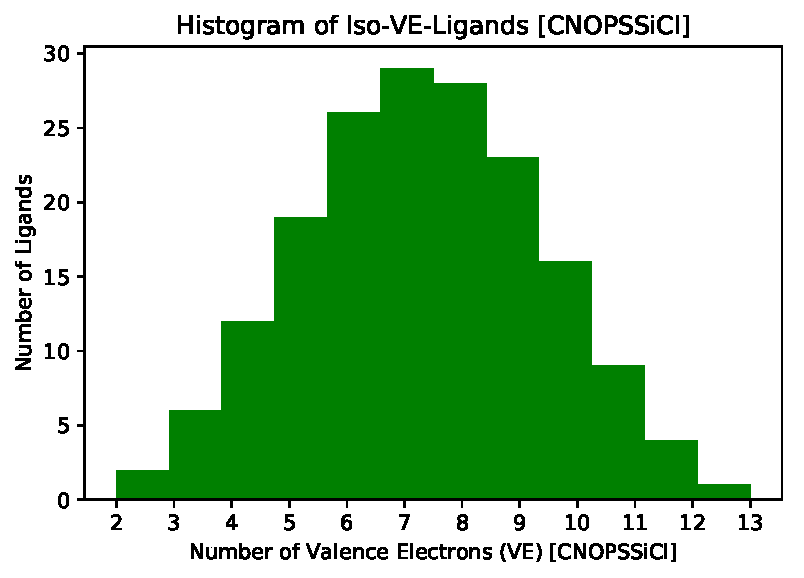
\includegraphics[width=.5\linewidth]{img/hist_isove_ligands_CNOPSSiCl.pdf} 
		\caption{CNOPSSiCl: 30625 ligands} 
		\vspace{4ex}
	\end{minipage} 
\end{figure}
\end{frame}

%------------------------------------------------

\begin{frame}
\frametitle{Now we go to Di-Heavy-Atomic Ligands ...}
\begin{itemize}
	\item Exhaustive combinatorial combination from the Mono-Heavy-Atomic Ligands to get Di-Heavy-Ligands
	\item Over heavy atoms identities $a_i \in \textrm{\{C,~N,~O,~P,~S,~(Si,~Cl)\}}$, charges $c_i \in \{-2, +2\}$, number of H atoms $h_i \in \{0, 4\}$, with heavy atoms $i \in {1,2}$, where $i=1$ is the coordinating atom.
	\item Pruned by means of a health function, $u$, of ligand $j$, to encoding heuristics.
\end{itemize}
\end{frame}

%------------------------------------------------

\begin{frame}
\frametitle{Now we go to Di-Heavy-Atomic Ligands ...}
\begin{itemize}
	\item Only ligands with $c_1 \leq 0 \wedge c_2 \leq 0$ are considered.
\end{itemize}
\begin{equation}
u_{\textrm{octet,i}} = 
\begin{cases}
10 + 2 \cdot (8-VE_i) 	& \mathrm{if}~ 8-VE_i < 0 \\
10 - 1 \cdot (8-VE_i) 	& \mathrm{if}~ 8-VE_i \geq 0
\end{cases}
\end{equation}

\begin{equation}
u_{\textrm{charge}} = 
\begin{cases}
0	&	\mathrm{if}~ c_1 + c_2 > 0 \\
3	&	\mathrm{if}~ 0 \geq c_1 + c_2 \geq -2 \\
1   &	\mathrm{if}~ c_1 + c_2 = -3 \\
0   &	\mathrm{if}~ c_1 + c_2 = -4 
\end{cases}
\end{equation}

\begin{equation}
u_{\textrm{VSEPR}} = 
 5-|\underbrace{(VE_1 - 2 \cdot LP_1 + c_1 - 2 \cdot h_1)}_{ready~electrons} -  \underbrace{(VE_2 - 2 \cdot LP_2 + c_2 - 2 \cdot h_2)}_{ready~electrons}|
\end{equation}
\end{frame}


%------------------------------------------------

\begin{frame}
\frametitle{Now we go to Di-Heavy-Atomic Ligands ...}

\begin{equation}
u_{\textrm{CA}} = 
\begin{cases}
1	&	\mathrm{if}~ h_1 = 4 \\
2	&	\mathrm{if}~ h_1 = 3 \\
3   &	\mathrm{if}~ \textrm{else} 
\end{cases}
\end{equation}

\begin{equation}
u_{\textrm{shell}} = 
\begin{cases}
1	&	\mathrm{if}~ \neg (VE_1+VE_2) \% 2 \\
0	&	\mathrm{if}~ \textrm{else}
\end{cases}
\end{equation}

\begin{equation}
u_{\textrm{total}} = u_{\textrm{shell}} \cdot \left( \frac{1}{2} ( u_{\textrm{octet,1}} + u_{\textrm{octet,i}} ) + u_{\textrm{charge}} + u_{\textrm{VSEPR}} + u_{\textrm{CA}} \right)
\end{equation}

where $VE_i$ denotes the number of valence electrons, $LP_i$ the number of lone pairs.
\end{frame}


%------------------------------------------------

\begin{frame}
\frametitle{Distribution of the Score}

\begin{table*}\centering
	\caption{Comparison of edge cases. Mayer B.O. with \texttt{multiwfn}.}
{
		\begin{tabular}{llccl}
			\toprule
			1         & 2       & Mayer B.O. & score & comment  \\
			\midrule
			CHHHH++ & CHHHH++&	$<$0.05 &12 & rather high  \\
			CHHHH-- & CHHHH--&	0.928 &-  & $c_{tot} > 0$  \\
			CHHH    & NH     &	1.308&0  & open shell  \\
			CH4++   & -        &	0.577&-  & Mono-Heavy-Atom\\
			C-      &O+     &	-    &16 & dummy \\
			\bottomrule
		\end{tabular}
	}
	
\end{table*}

\end{frame}

%------------------------------------------------

\begin{frame}
\frametitle{Distribution of the Score}
\begin{figure}
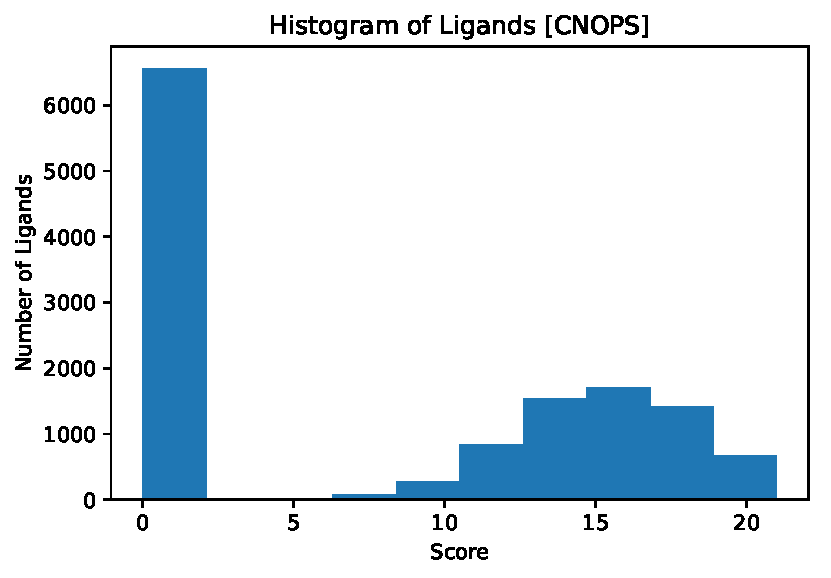
\includegraphics[width=0.7\linewidth]{img/distr_CNOPS.pdf}
\caption{A histogram describing the score distribution. There are 30 ligands with score 21 and 180 ligands with score 20. CO is has a score of 16. There are 2917 ligands at least as good as CO.} 
\end{figure}
\end{frame}

%------------------------------------------------

\begin{frame}
\frametitle{Code Output}
\texttt{\tiny{[['[NHH-]', 10, 8, 1, -1, 2, 0, 1, 10, '[CHHH-]', 10, 8, 0, -1, 3, 0, 1, 10], 21.0]\\
[['[NHH-]', 10, 8, 1, -1, 2, 0, 1, 10, '[NHH-]', 10, 8, 1, -1, 2, 0, 1, 10], 21.0]\\
[['[NHH-]', 10, 8, 1, -1, 2, 0, 1, 10, '[OH-]', 10, 8, 2, -1, 1, 0, 1, 10], 21.0]\\
[['[NHH-]', 10, 8, 1, -1, 2, 0, 1, 10, '[PHH-]', 18, 8, 1, -1, 2, 0, 1, 10], 21.0]\\
[['[NHH-]', 10, 8, 1, -1, 2, 0, 1, 10, '[SH-]', 18, 8, 2, -1, 1, 0, 1, 10], 21.0]\\
[['[OH-]', 10, 8, 2, -1, 1, 0, 1, 10, '[CHHH-]', 10, 8, 0, -1, 3, 0, 1, 10], 21.0]\\
[['[OHH]', 10, 8, 2, 0, 2, 0, 1, 10, '[CHHHH]', 10, 8, 0, 0, 4, 0, 1, 10], 21.0]\\
[['[OH-]', 10, 8, 2, -1, 1, 0, 1, 10, '[NHH-]', 10, 8, 1, -1, 2, 0, 1, 10], 21.0]\\
[['[OHH]', 10, 8, 2, 0, 2, 0, 1, 10, '[NHHH]', 10, 8, 1, 0, 3, 0, 1, 10], 21.0]\\
[['[OH-]', 10, 8, 2, -1, 1, 0, 1, 10, '[OH-]', 10, 8, 2, -1, 1, 0, 1, 10], 21.0]\\
[['[OHH]', 10, 8, 2, 0, 2, 0, 1, 10, '[OHH]', 10, 8, 2, 0, 2, 0, 1, 10], 21.0]\\}}
\end{frame}

%%------------------------------------------------
%
%\begin{frame}
%\frametitle{Bullet Points}
%\begin{itemize}
%\item Lorem ipsum dolor sit amet, consectetur adipiscing elit
%\item Aliquam blandit faucibus nisi, sit amet dapibus enim tempus eu
%\item Nulla commodo, erat quis gravida posuere, elit lacus lobortis est, quis porttitor odio mauris at libero
%\item Nam cursus est eget velit posuere pellentesque
%\item Vestibulum faucibus velit a augue condimentum quis convallis nulla gravida
%\end{itemize}
%\end{frame}
%
%%------------------------------------------------
%
%\begin{frame}
%\frametitle{Blocks of Highlighted Text}
%\begin{block}{Block 1}
%Lorem ipsum dolor sit amet, consectetur adipiscing elit. Integer lectus nisl, ultricies in feugiat rutrum, porttitor sit amet augue. Aliquam ut tortor mauris. Sed volutpat ante purus, quis accumsan dolor.
%\end{block}
%
%\begin{block}{Block 2}
%Pellentesque sed tellus purus. Class aptent taciti sociosqu ad litora torquent per conubia nostra, per inceptos himenaeos. Vestibulum quis magna at risus dictum tempor eu vitae velit.
%\end{block}
%
%\begin{block}{Block 3}
%Suspendisse tincidunt sagittis gravida. Curabitur condimentum, enim sed venenatis rutrum, ipsum neque consectetur orci, sed blandit justo nisi ac lacus.
%\end{block}
%\end{frame}
%
%%------------------------------------------------
%
%\begin{frame}
%\frametitle{Multiple Columns}
%\begin{columns}[c] % The "c" option specifies centered vertical alignment while the "t" option is used for top vertical alignment
%
%\column{.45\textwidth} % Left column and width
%\textbf{Heading}
%\begin{enumerate}
%\item Statement
%\item Explanation
%\item Example
%\end{enumerate}
%
%\column{.5\textwidth} % Right column and width
%Lorem ipsum dolor sit amet, consectetur adipiscing elit. Integer lectus nisl, ultricies in feugiat rutrum, porttitor sit amet augue. Aliquam ut tortor mauris. Sed volutpat ante purus, quis accumsan dolor.
%
%\end{columns}
%\end{frame}
%
%%------------------------------------------------
%\section{Second Section}
%%------------------------------------------------
%
%\begin{frame}
%\frametitle{Table}
%\begin{table}
%\begin{tabular}{l l l}
%\toprule
%\textbf{Treatments} & \textbf{Response 1} & \textbf{Response 2}\\
%\midrule
%Treatment 1 & 0.0003262 & 0.562 \\
%Treatment 2 & 0.0015681 & 0.910 \\
%Treatment 3 & 0.0009271 & 0.296 \\
%\bottomrule
%\end{tabular}
%\caption{Table caption}
%\end{table}
%\end{frame}
%
%%------------------------------------------------
%
%\begin{frame}
%\frametitle{Theorem}
%\begin{theorem}[Mass--energy equivalence]
%$E = mc^2$
%\end{theorem}
%\end{frame}
%
%%------------------------------------------------
%
%\begin{frame}[fragile] % Need to use the fragile option when verbatim is used in the slide
%\frametitle{Verbatim}
%\begin{example}[Theorem Slide Code]
%\begin{verbatim}
%\begin{frame}
%\frametitle{Theorem}
%\begin{theorem}[Mass--energy equivalence]
%$E = mc^2$
%\end{theorem}
%\end{frame}\end{verbatim}
%\end{example}
%\end{frame}
%
%%------------------------------------------------
%
%\begin{frame}
%\frametitle{Figure}
%Uncomment the code on this slide to include your own image from the same directory as the template .TeX file.
%%\begin{figure}
%%\includegraphics[width=0.8\linewidth]{test}
%%\end{figure}
%\end{frame}
%
%%------------------------------------------------
%
%\begin{frame}[fragile] % Need to use the fragile option when verbatim is used in the slide
%\frametitle{Citation}
%An example of the \verb|\cite| command to cite within the presentation:\\~
%
%This statement requires citation \cite{p1}.
%\end{frame}
%
%%------------------------------------------------
%
%\begin{frame}
%\frametitle{References}
%\footnotesize{
%\begin{thebibliography}{99} % Beamer does not support BibTeX so references must be inserted manually as below
%\bibitem[Smith, 2012]{p1} John Smith (2012)
%\newblock Title of the publication
%\newblock \emph{Journal Name} 12(3), 45 -- 678.
%\end{thebibliography}
%}
%\end{frame}
%
%%------------------------------------------------
%
%\begin{frame}
%\Huge{\centerline{The End}}
%\end{frame}
%
%%----------------------------------------------------------------------------------------

\end{document}